%% Compile: pdflatex > pdflatex (no biber needed; references are hardcoded for presentation)
%% For speaker notes in a separate PDF: uncomment \setbeameroption{show notes on second screen=right}

\documentclass[aspectratio=169, 11pt]{beamer}

\usepackage[utf8]{inputenc}
\usepackage[T1]{fontenc}
\usepackage{lmodern}
\usepackage[british]{babel}

\usepackage{amsmath,amssymb}
\usepackage{booktabs}
\usepackage{array}
\usepackage{graphicx}
\usepackage{tikz}
\usetikzlibrary{positioning, arrows, calc, shapes.geometric,
  fit, backgrounds, decorations.pathreplacing, decorations.pathmorphing}
\usepackage{appendixnumberbeamer}
\usepackage{pgfpages}

% Uncomment for dual-screen speaker notes:
% \setbeameroption{show notes on second screen=right}

\definecolor{Navy}{HTML}{0D1B2A}
\definecolor{MidNavy}{HTML}{1B2E4A}
\definecolor{DkOrange}{HTML}{D97706}
\definecolor{LtOrange}{HTML}{F5DEB3}
\definecolor{Bordeaux}{HTML}{7A1C2E}
\definecolor{BordeauxLt}{HTML}{A63D50}
\definecolor{Ivory}{HTML}{FAF8F5}
\definecolor{WarmGrey}{HTML}{E8E4DF}
\definecolor{MidGrey}{HTML}{9CA3AF}
\definecolor{DkGrey}{HTML}{4B5563}
\definecolor{Teal}{HTML}{2A7F8C}
\definecolor{TealLt}{HTML}{D0ECF0}
\definecolor{ForestGreen}{HTML}{4A7C59}

\usefonttheme{professionalfonts}
\setbeamercolor{normal text}{fg=Navy, bg=Ivory}
\setbeamercolor{alerted text}{fg=Bordeaux}
\setbeamercolor{example text}{fg=DkOrange}

% Frame title
\setbeamercolor{frametitle}{fg=Ivory, bg=Navy}
\setbeamerfont{frametitle}{size=\large, series=\bfseries}
\setbeamertemplate{frametitle}{%
  \nointerlineskip
  \begin{beamercolorbox}[wd=\paperwidth, ht=2.6em, dp=0.8em, leftskip=1.2em]{frametitle}%
    \usebeamerfont{frametitle}\insertframetitle%
  \end{beamercolorbox}%
  {\color{DkOrange}\hrule height 2.2pt}%
}

% Title page
\setbeamercolor{title}{fg=Ivory}
\setbeamercolor{subtitle}{fg=LtOrange}
\setbeamercolor{author}{fg=Ivory}
\setbeamercolor{date}{fg=WarmGrey}
\setbeamercolor{institute}{fg=WarmGrey}
\setbeamerfont{title}{size=\Large, series=\bfseries}
\setbeamerfont{subtitle}{size=\normalsize, shape=\itshape}

% Itemize
\setbeamertemplate{itemize item}{\color{DkOrange}\scriptsize$\blacksquare$}
\setbeamertemplate{itemize subitem}{\color{Bordeaux}\scriptsize$\blacktriangleright$}
\setbeamercolor{itemize item}{fg=DkOrange}
\setbeamercolor{itemize subitem}{fg=Bordeaux}

% Footer
\setbeamertemplate{navigation symbols}{}
\setbeamertemplate{footline}{%
  \hfill
  \raisebox{3pt}{\color{MidGrey}\scriptsize\insertframenumber\,/\,\inserttotalframenumber}%
  \hspace{8pt}\vspace{3pt}%
}

% Blocks
\setbeamercolor{block title}{fg=Ivory, bg=MidNavy}
\setbeamercolor{block body}{fg=Navy, bg=WarmGrey}
\setbeamercolor{block title alerted}{fg=Ivory, bg=Bordeaux}
\setbeamercolor{block body alerted}{fg=Navy, bg=WarmGrey}
\setbeamercolor{block title example}{fg=Ivory, bg=DkOrange}
\setbeamercolor{block body example}{fg=Navy, bg=WarmGrey}
\setbeamerfont{block title}{series=\bfseries}

% Section page
\AtBeginSection[]{%
  \begin{frame}
    \vfill
    \centering
    {\color{Navy}\Huge\bfseries\insertsectionnumber}\\[0.6em]
    {\color{Navy}\LARGE\bfseries\insertsectionhead}\\[0.4em]
    {\color{DkOrange}\rule{4cm}{2pt}}
    \vfill
  \end{frame}
}

\newcommand{\highlight}[1]{\textcolor{DkOrange}{\textbf{#1}}}
\newcommand{\emphbx}[1]{\textcolor{Bordeaux}{\textbf{#1}}}
\newcommand{\EUR}{\texteuro}

\newcolumntype{L}[1]{>{\raggedright\arraybackslash}p{#1}}
\newcolumntype{C}[1]{>{\centering\arraybackslash}p{#1}}


\title{Decomposition of Global Minimum Tax Revenue\\Using CbCR Data}
\subtitle{A factorial decomposition for quantifying uncertainty\\in EU revenue estimates under Pillar Two}
\author{Maurits de Haan}
\institute{MSc Economic Policy\\ Utrecht University School of Economics}
\date{April 2026}

\begin{document}

{
\setbeamercolor{background canvas}{bg=Navy}
\begin{frame}[plain]
  \vspace{1.8em}
  \begin{center}
    {\color{Ivory}\Large\bfseries Decomposition of Global Minimum Tax Revenue}\\[0.3em]
    {\color{Ivory}\Large\bfseries using CbCR Data}\\[0.8em]
    {\color{DkOrange}\rule{6cm}{2pt}}\\[0.8em]
    {\color{LtOrange}\normalsize\itshape A factorial decomposition for quantifying uncertainty\\[0.2em]
     in EU revenue estimates under Pillar Two}\\[1.8em]
    {\color{Ivory}\normalsize Maurits de Haan}\\[0.3em]
    {\color{WarmGrey}\small MSc Economic Policy, Utrecht University}\\[0.3em]
    {\color{WarmGrey}\small Supervisor: dr.\ Peter Gerbrands \quad Second reader: dr.\ Adriaan Kalwij}\\[1.2em]
    {\color{MidGrey}\small 13 April 2026}
  \end{center}
\end{frame}
}

\section{The problem and relevance}

\begin{frame}{The Global Minimum Tax in one picture}
\begin{center}
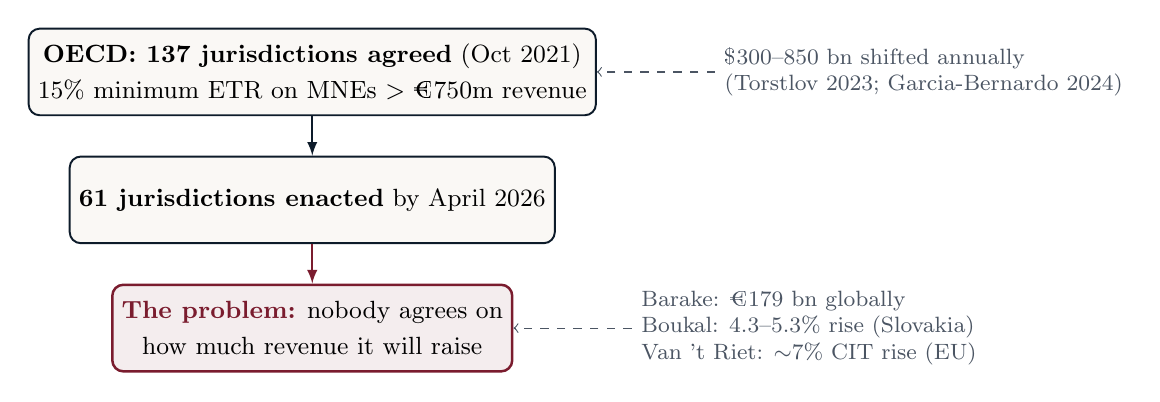
\begin{tikzpicture}[font=\small, node distance=0.7cm]
  % Fact boxes
  \node[draw=Navy, rounded corners=4pt, fill=Ivory, line width=0.7pt,
        minimum width=5cm, minimum height=1.1cm, align=center] (f1)
    {\textbf{OECD: 137 jurisdictions agreed} (Oct 2021)\\[2pt]
     15\% minimum ETR on MNEs $>$ \EUR750m revenue};

  \node[draw=Navy, rounded corners=4pt, fill=Ivory, line width=0.7pt,
        minimum width=5cm, minimum height=1.1cm, align=center,
        below=0.5cm of f1] (f2)
    {\textbf{61 jurisdictions enacted} by April 2026};

  \node[draw=Bordeaux, rounded corners=4pt, fill=Bordeaux!8, line width=0.9pt,
        minimum width=5cm, minimum height=1.1cm, align=center,
        below=0.5cm of f2] (f3)
    {\emphbx{The problem:} nobody agrees on\\[2pt]
     how much revenue it will raise};

  \draw[-latex, Navy, line width=0.7pt] (f1) -- (f2);
  \draw[-latex, Bordeaux, line width=0.7pt] (f2) -- (f3);

  % Right side: numbers
  \node[right=1.5cm of f1, align=left, font=\footnotesize, text=DkGrey] (n1)
    {\$300--850 bn shifted annually\\(Torstlov 2023; Garcia-Bernardo 2024)};
  \node[right=1.5cm of f3, align=left, font=\footnotesize, text=DkGrey] (n2)
    {Barake: \EUR179 bn globally\\Boukal: 4.3--5.3\% rise (Slovakia)\\Van 't Riet: $\sim$7\% CIT rise (EU)};

  \draw[->, DkGrey, line width=0.4pt, dashed] (n1.west) -- (f1.east);
  \draw[->, DkGrey, line width=0.4pt, dashed] (n2.west) -- (f3.east);
\end{tikzpicture}
\end{center}

\vspace{0.6em}
\highlight{Revenue estimates diverge}, and nobody has shown \emph{why} they diverge.
\end{frame}

\begin{frame}{Societal relevance: governments budget on guesswork}
\begin{block}{The Dutch case}
  The Netherlands projected \highlight{\EUR466 million} in annual GMT revenue.\\[6pt]
  \emphbx{86\%} of that comes from a single assumption: the behavioural response (profit that MNEs stop shifting).\\[6pt]
  The January 2026 Side-by-Side package implies a \highlight{\EUR122 million} annual revenue loss.
\end{block}
\vspace{0.5em}
Finance ministries across the EU face the same uncertainty. Fiscal plans rest on untested assumptions.
\end{frame}


\begin{frame}{Scientific relevance: four gaps in the literature}
\begin{enumerate}
  \item \emphbx{No panel semi-elasticity:} Dowd (2017): US-only. Garcia-Bernardo (2024): single cross-section 2017. Neither uses the 2016--2022 CbCR panel with bilateral fixed effects.

  \item \emphbx{No factorial decomposition:} Barake et. al. (2022) and Hugger (2026) vary parameters one at a time. Interactions between modelling choices are invisible.

  \item \emphbx{No CbCR $\times$ FATS sectoral analysis:} The SBIE depends on sectoral payroll and assets. No study combines CbCR aggregate levels with FATS sectoral shares.

  \item \emphbx{No cross-validation of the ETR distribution:} CbCR Table I percentiles vs.\ Table IV direct observation. Nobody has tested whether the five-percentile fit recovers the actual low-taxed profit share.
\end{enumerate}
\end{frame}

\section{Where does the literature stand now?}

\begin{frame}{Three sources of divergence in revenue estimates}
\begin{center}
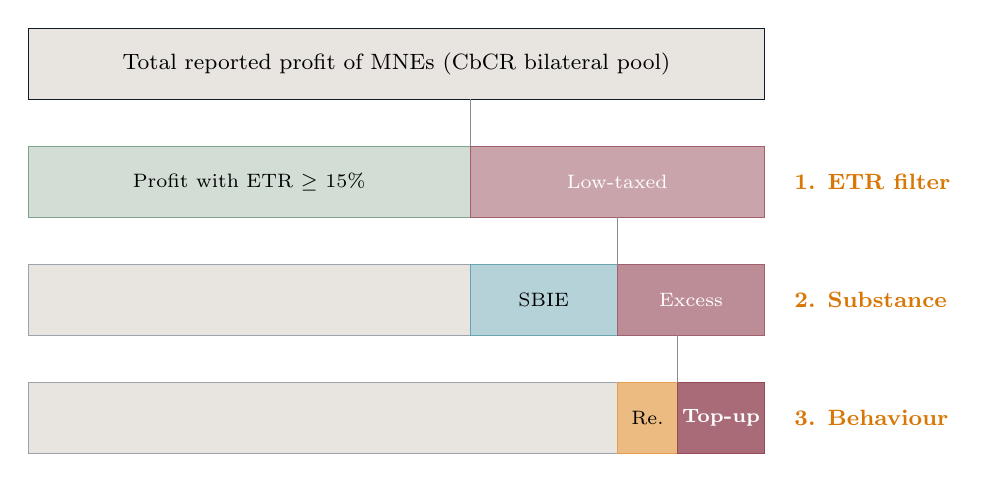
\begin{tikzpicture}[font=\small, xscale=0.85]
  \def\tw{11}
  \def\th{0.9}

  % Layer 1
  \fill[WarmGrey, draw=Navy, line width=0.5pt] (0,3.5) rectangle (\tw, 3.5+\th);
  \node[font=\footnotesize] at (\tw/2, 3.5+\th/2) {Total reported profit of MNEs (CbCR bilateral pool)};

  % Layer 2
  \fill[ForestGreen!25, draw=ForestGreen!70] (0,2.0) rectangle (6.6, 2.0+\th);
  \fill[Bordeaux!40, draw=Bordeaux!70] (6.6,2.0) rectangle (\tw, 2.0+\th);
  \node[font=\scriptsize, align=center] at (3.3, 2.0+\th/2) {Profit with ETR $\geq$ 15\%};
  \node[font=\scriptsize, white] at (8.8, 2.0+\th/2) {Low-taxed};
  \node[font=\footnotesize, DkOrange, anchor=west] at (\tw+0.3, 2.0+\th/2) {\textbf{1. ETR filter}};

  % Layer 3
  \fill[WarmGrey, draw=MidGrey] (0,0.5) rectangle (6.6, 0.5+\th);
  \fill[Teal!35, draw=Teal!70] (6.6,0.5) rectangle (8.8, 0.5+\th);
  \fill[Bordeaux!50, draw=Bordeaux!70] (8.8,0.5) rectangle (\tw, 0.5+\th);
  \node[font=\scriptsize] at (7.7, 0.5+\th/2) {SBIE};
  \node[font=\scriptsize, white] at (9.9, 0.5+\th/2) {Excess};
  \node[font=\footnotesize, DkOrange, anchor=west] at (\tw+0.3, 0.5+\th/2) {\textbf{2. Substance}};

  % Layer 4
  \fill[WarmGrey, draw=MidGrey] (0,-1.0) rectangle (8.8, -1.0+\th);
  \fill[DkOrange!50, draw=DkOrange!70] (8.8,-1.0) rectangle (9.7, -1.0+\th);
  \fill[Bordeaux!65, draw=Bordeaux!80] (9.7,-1.0) rectangle (\tw, -1.0+\th);
  \node[font=\scriptsize] at (9.25, -1.0+\th/2) {Re.};
  \node[font=\scriptsize, white, align=center] at (10.35, -1.0+\th/2) {\textbf{Top-up}};
  \node[font=\footnotesize, DkOrange, anchor=west] at (\tw+0.3, -1.0+\th/2) {\textbf{3. Behaviour}};

  % Connectors
  \draw[Navy!50, line width=0.3pt] (6.6, 3.5) -- (6.6, 2.0+\th);
  \draw[Navy!50, line width=0.3pt] (8.8, 2.0) -- (8.8, 0.5+\th);
  \draw[Navy!50, line width=0.3pt] (9.7, 0.5) -- (9.7, -1.0+\th);
\end{tikzpicture}
\end{center}
\end{frame}

\begin{frame}{Key finding from the literature: within-jurisdiction heterogeneity}
\begin{columns}[T]
\begin{column}{0.55\textwidth}
  Hugger (2026) demonstrates that \highlight{53.2\%} of all low-taxed profit sits in jurisdictions where the \emph{average} ETR is above 15\%.\\[10pt]

  Jurisdiction-average approaches (Barake 2022) therefore \emphbx{miss more than half} of the GMT base.\\[10pt]

  The distributional approach uses five ETR percentiles from CbCR Table I to reconstruct within-jurisdiction variation.
\end{column}
\begin{column}{0.42\textwidth}
\vspace{0.5em}
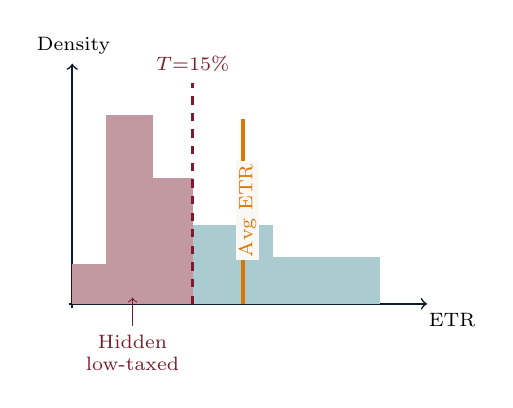
\begin{tikzpicture}[font=\small, xscale=0.85]
  % Simplified ETR density
  \draw[->, Navy, line width=0.6pt] (-0.05,0) -- (5.3,0);
  \draw[->, Navy, line width=0.6pt] (0,-0.05) -- (0,3.05);
  \node[font=\scriptsize, anchor=north west] at (5.18,0.0) {ETR};
  \node[font=\scriptsize, anchor=south] at (0.02,3.05) {Density};

  % Bars (low-taxed in Bordeaux, above-15 in Teal)
  \fill[Bordeaux!45] (0,0) rectangle (0.5, 0.5);
  \fill[Bordeaux!45] (0.5,0) rectangle (1.2, 2.4);
  \fill[Bordeaux!45] (1.2,0) rectangle (1.8, 1.6);
  \fill[Teal!40] (1.8,0) rectangle (3.0, 1.0);
  \fill[Teal!40] (3.0,0) rectangle (4.6, 0.6);

  % Threshold
  \draw[Bordeaux, dashed, line width=1pt] (1.8,0) -- (1.8,2.8);
  \node[font=\scriptsize, Bordeaux, anchor=south] at (1.8,2.82) {$T{=}15\%$};

  % Average ETR line
  \draw[DkOrange, line width=1.2pt] (2.55,0) -- (2.55,2.35);
  \node[font=\scriptsize, DkOrange, rotate=90, anchor=west, fill=Ivory, inner sep=1pt] at (2.62,0.55) {Avg ETR};

  % Annotation
  \node[font=\scriptsize, Bordeaux, align=center] at (0.9, -0.62) {Hidden\\low-taxed};
  \draw[->, Bordeaux, line width=0.4pt] (0.9, -0.28) -- (0.9, 0.08);
\end{tikzpicture}
\end{column}
\end{columns}
\end{frame}

\begin{frame}{Nonlinear profit shifting: semi-elasticity at low rates}
\begin{columns}[T]
\begin{column}{0.52\textwidth}
  The semi-elasticity of profits with respect to tax rates is \emphbx{not constant}:\\[8pt]

  \begin{tabular}{@{}lcc@{}}
    \toprule
    & \textbf{At 5\%} & \textbf{At 30\%} \\
    \midrule
    Consensus (H\&R) & 0.8 & 0.8 \\
    Dowd (quadratic) & 4.7 & 0.7 \\
    Garcia-B.\ (log) & $>$5 & $\sim$0.6 \\
    \bottomrule
  \end{tabular}\\[10pt]

  At low rates --- where the GMT bites --- the response is \highlight{5--6$\times$ larger} than the consensus.\\[8pt]
  No panel estimate exists with bilateral fixed effects.
\end{column}
\begin{column}{0.45\textwidth}
\vspace{0.3em}
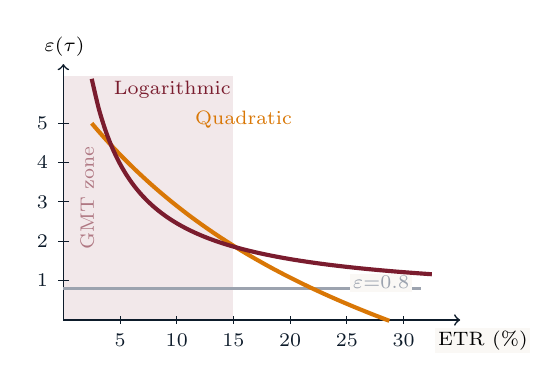
\begin{tikzpicture}[font=\small, xscale=0.72, yscale=0.5]
  % GMT zone background (draw first)
  \fill[Bordeaux!10] (0,0) rectangle (3, 6.2);

  % Axes
  \draw[->, Navy, line width=0.6pt] (0,0) -- (7.0,0);
  \draw[->, Navy, line width=0.6pt] (0,0) -- (0,6.5);
  \node[font=\scriptsize, anchor=west, fill=Ivory, inner sep=1pt] at (6.55,-0.52) {ETR (\%)};
  \node[font=\scriptsize, anchor=south] at (0.02,6.45) {$\varepsilon(\tau)$};

  % Ticks
  \foreach \x/\lbl in {1/5, 2/10, 3/15, 4/20, 5/25, 6/30} {
    \draw[Navy] (\x, 0.1) -- (\x, -0.1) node[below, font=\scriptsize] {\lbl};
  }
  \foreach \y/\lbl in {1/1, 2/2, 3/3, 4/4, 5/5} {
    \draw[Navy] (0.1, \y) -- (-0.1, \y) node[left, font=\scriptsize] {\lbl};
  }

  % Constant (consensus)
  \draw[MidGrey, line width=1.2pt] (0, 0.8) -- (6.3, 0.8);
  \node[font=\scriptsize, MidGrey, anchor=west, fill=Ivory, inner sep=1pt] at (5.05, 0.95) {$\varepsilon{=}0.8$};

  % Quadratic (Dowd)
  \draw[DkOrange, line width=1.5pt, smooth, domain=0.5:5.75, samples=50]
    plot (\x, {-0.73 + 1.6178*(6-\x)/5 + 4.7*exp(-0.35*\x)});
  \node[font=\scriptsize, DkOrange, anchor=west] at (2.15, 5.1) {Quadratic};

  % Log (Garcia-Bernardo)
  \draw[Bordeaux, line width=1.5pt, smooth, domain=0.5:6.5, samples=50]
    plot (\x, {0.5 + 4.5/(0.3+\x)});
  \node[font=\scriptsize, Bordeaux, anchor=west] at (0.72, 5.85) {Logarithmic};

  % GMT zone label
  \node[font=\scriptsize, Bordeaux!60, rotate=90] at (0.42, 3.1) {GMT zone};
\end{tikzpicture}
\end{column}
\end{columns}
\end{frame}

\note{
The behavioural response is the second big driver. The consensus semi-elasticity is 0.8, but that is an average across the whole tax distribution. Dowd shows it is 4.7 at a 5 percent rate --- nearly six times larger. Garcia-Bernardo's logarithmic specification goes even higher. The GMT zone on the left of the graph is exactly where the nonlinearity matters most. I estimate this on a seven-year panel with pair fixed effects, which has not been done before. This is subquestion 1.
}


%% ═══════════════════════════════════════════════
\section{What Do I Do Differently?}
%% ═══════════════════════════════════════════════

\begin{frame}{Research question}
\begin{alertblock}{}
\itshape
What profit-shifting semi-elasticities emerge from the 2016--2022 CbCR panel under different functional forms, and how sensitive are the resulting Global Minimum Tax revenue estimates for EU Member States to the measurement of effective tax rates, the substance-based income exclusion, the implementation of the Side-by-Side package, and the specification of behavioural responses?
\end{alertblock}

\vspace{0.8em}
\textbf{Three subquestions:}
\begin{enumerate}
  \item \highlight{Estimate} the semi-elasticity (linear, quadratic, logarithmic) on 2016--2022 CbCR with bilateral FE
  \item \highlight{Decompose} revenue variation through a $2^5$ factorial design over five modelling choices
  \item \highlight{Quantify} the Side-by-Side and SBTI Safe Harbour effects on EU revenue and collection channels
\end{enumerate}
\end{frame}

\note{
This is the research question. Three subquestions. SQ1 estimates the semi-elasticity on the panel. SQ2 runs the full factorial decomposition with ANOVA. SQ3 quantifies the January 2026 policy changes. Together they tell finance ministries which assumptions drive which numbers.
}


\begin{frame}{The revenue pipeline: three multiplicative filters}
\begin{center}
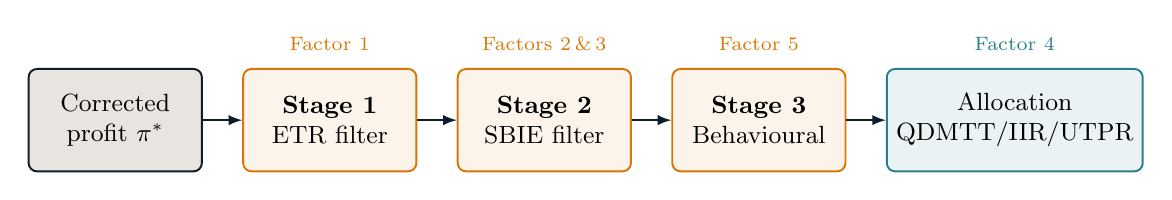
\begin{tikzpicture}[font=\small, node distance=0.6cm]
  % Styles
  \tikzset{
    stage/.style={draw=Navy, line width=0.7pt, rounded corners=3pt,
      fill=WarmGrey, minimum width=2.2cm, minimum height=1.3cm, align=center},
    filt/.style={draw=DkOrange, line width=0.7pt, rounded corners=3pt,
      fill=DkOrange!8, minimum width=2.2cm, minimum height=1.3cm, align=center},
    alloc/.style={draw=Teal, line width=0.7pt, rounded corners=3pt,
      fill=Teal!10, minimum width=2.2cm, minimum height=1.3cm, align=center},
    arr/.style={-latex, draw=Navy, line width=0.7pt}
  }

  \node[stage] (input) {Corrected\\profit $\pi^{*}$};
  \node[filt, right=0.5cm of input] (s1) {\textbf{Stage 1}\\ETR filter};
  \node[filt, right=0.5cm of s1] (s2) {\textbf{Stage 2}\\SBIE filter};
  \node[filt, right=0.5cm of s2] (s3) {\textbf{Stage 3}\\Behavioural};
  \node[alloc, right=0.5cm of s3] (alloc) {Allocation\\QDMTT/IIR/UTPR};

  \draw[arr] (input) -- (s1);
  \draw[arr] (s1) -- (s2);
  \draw[arr] (s2) -- (s3);
  \draw[arr] (s3) -- (alloc);

  % Factor labels
  \node[font=\scriptsize, DkOrange, above=0.1cm of s1] {Factor 1};
  \node[font=\scriptsize, DkOrange, above=0.1cm of s2] {Factors 2\,\&\,3};
  \node[font=\scriptsize, DkOrange, above=0.1cm of s3] {Factor 5};
  \node[font=\scriptsize, Teal, above=0.1cm of alloc] {Factor 4};
\end{tikzpicture}
\end{center}

\vspace{0.4em}
$$
L_{p,j,t} = \underbrace{s_{j,t}^{<T}\, \pi_{p,j,t}^{*}\, \bar{\delta}_{j,t}^{\text{top}}}_{\text{Stage 1}} \times \underbrace{(1 - \bar{\phi}_{p,j,t})}_{\text{Stage 2}} \times \underbrace{(1 - \beta_{j,t})}_{\text{Stage 3}}
$$

\vspace{0.4em}
{\footnotesize Each factor has two levels $\to$ $2^5 = 32$ scenarios $\to$ ANOVA decomposes the variance exactly.}
\end{frame}

\note{
Here is the pipeline. Corrected profits flow through three multiplicative stages. Stage 1 identifies the low-taxed share and the average top-up rate. Stage 2 applies the substance exclusion. Stage 3 applies the behavioural response. The result is allocated across QDMTT, IIR, and UTPR. Five binary factors generate 32 scenarios. An ANOVA identity decomposes the variance into main effects and interactions. The key equation is on screen: everything multiplies. That is why interactions matter.
}


\begin{frame}{The $2^5$ factorial design}
\begin{center}
\footnotesize
\begin{tabular}{@{}L{0.7cm}L{3.8cm}L{3.5cm}L{3.8cm}@{}}
  \toprule
  & \textbf{Factor} & \textbf{Level 0} & \textbf{Level 1} \\
  \midrule
  $x_1$ & ETR measurement & Jurisdiction-average & Within-jurisdiction distributional \\[2pt]
  $x_2$ & Substance specification & Aggregate SBIE & Sectoral SBIE + SBTI overlay \\[2pt]
  $x_3$ & SBIE carve-out rates & Initial (10\%/8\%) & Long-run (5\%/5\%) \\[2pt]
  $x_4$ & Implementation regime & Universal IIR/UTPR & Side-by-Side Safe Harbour \\[2pt]
  $x_5$ & Behavioural response & None ($\beta = 0$) & Panel-estimated semi-elasticity \\
  \bottomrule
\end{tabular}
\end{center}

\vspace{0.3em}
The ANOVA identity decomposes total variance exactly:
$$
\text{SS}_{\text{total}} = \sum_{i} \text{SS}_i + \sum_{i<k} \text{SS}_{ik} + \cdots + \text{SS}_{12345}
$$

\vspace{-0.3em}
$\eta_i^2 = \text{SS}_i / \text{SS}_{\text{total}}$ tells us \highlight{which assumption matters most}.
\end{frame}

\note{
Here are the five factors. Each has two levels. ETR measurement is the biggest one conceptually: average versus distributional. The substance factor switches between an aggregate SBIE and a sectoral one that uses FATS data. Carve-out rates switch between initial (generous) and long-run (tight). The SbS factor captures the January 2026 policy package. And the behavioural factor switches between no response and the panel-estimated response. 32 scenarios. The ANOVA identity decomposes the total sum of squares exactly into main effects and all interactions. Eta-squared tells us which assumption drives which share of the variation.
}


%% ═══════════════════════════════════════════════
\section{Data}
%% ═══════════════════════════════════════════════

\begin{frame}{OECD CbCR data: two complementary tables}
\begin{center}
\small
\begin{tabular}{@{}L{3.5cm}C{4.0cm}C{4.0cm}@{}}
  \toprule
  & \textbf{Table I} & \textbf{Table IV} \\
  \midrule
  Aggregation & Bilateral totals & ETR brackets (subsidiary) \\
  Parent jurisdictions & 58 & 49 \\
  Affiliate jurisdictions & 240 & 154 \\
  Years & 2016--2022 & 2016--2022 \\
  EU-27 covered? & All 27 & All 27 \\[4pt]
  \highlight{Key feature} & 5 ETR percentiles & Direct \texttt{RATE\_0-15} bracket \\[4pt]
  Role in pipeline & Distributional fit & Direct observation + validation \\
  \bottomrule
\end{tabular}
\end{center}

\vspace{0.5em}
\textbf{Hybrid strategy:} use Table IV where observed (all EU), Table I distributional fit elsewhere. Cross-validate on the overlap.
\end{frame}

\note{
Two tables from the OECD CbCR. Table I has broader coverage and the five ETR percentiles I need for the distributional fit. Table IV has narrower coverage but directly observes the profit in the 0-to-15 percent bracket --- exactly the GMT base. All 27 EU Member States appear in both. So I use Table IV directly for the EU sample and the distributional fit from Table I for non-EU affiliates. The overlap lets me cross-validate: I can check whether the five-percentile fit actually recovers what Table IV observes. Nobody has done this test.
}


\begin{frame}{Eurostat FATS: the sectoral dimension CbCR lacks}
\begin{columns}[T]
\begin{column}{0.55\textwidth}
  CbCR reports \emph{no} sectoral breakdown.\\[8pt]
  The SBIE depends on payroll and tangible assets, which vary dramatically by sector:\\[6pt]
  \begin{itemize}
    \item Manufacturing: high substance $\to$ large SBIE
    \item IP licensing: near-zero substance $\to$ small SBIE
  \end{itemize}

  \vspace{8pt}
  \textbf{Solution:} FATS supplies sectoral \emph{shares}, CbCR supplies aggregate \emph{levels}.\\[6pt]
  Their product: sector-specific SBIE-to-profit ratios for 27 EU $\times$ 15--20 NACE sectors.
\end{column}
\begin{column}{0.42\textwidth}
\vspace{0.5em}
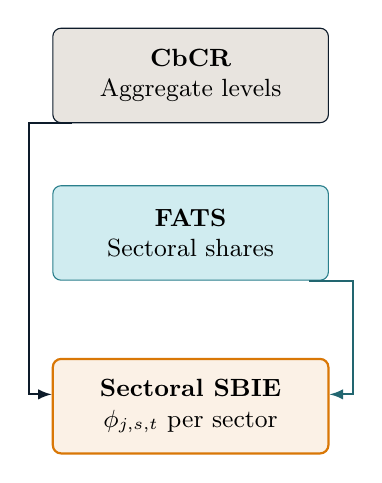
\begin{tikzpicture}[font=\small]
  % CbCR box
  \node[draw=Navy, rounded corners=3pt, fill=WarmGrey, minimum width=3.5cm,
        minimum height=1.2cm, align=center] (cbcr) at (0,3.0)
    {\textbf{CbCR}\\Aggregate levels};

  % FATS box
  \node[draw=Teal, rounded corners=3pt, fill=TealLt, minimum width=3.5cm,
        minimum height=1.2cm, align=center] (fats) at (0,1.0)
    {\textbf{FATS}\\Sectoral shares};

  % Combined
  \node[draw=DkOrange, rounded corners=3pt, fill=DkOrange!10, minimum width=3.5cm,
        minimum height=1.2cm, align=center, line width=0.8pt] (combo) at (0,-1.2)
    {\textbf{Sectoral SBIE}\\$\phi_{j,s,t}$ per sector};

  \draw[-latex, Navy, line width=0.7pt]
    ([xshift=0.25cm]cbcr.south west) -- ++(-0.55,0)
    |- ([yshift=0.15cm]combo.west);

  \draw[-latex, Teal!80!black, line width=0.7pt]
    ([xshift=-0.25cm]fats.south east) -- ++(0.55,0)
    |- ([yshift=0.15cm]combo.east);
\end{tikzpicture}
\end{column}
\end{columns}
\end{frame}

\note{
CbCR has no sectors. But the SBIE depends on payroll and tangible assets, which vary enormously by sector. Manufacturing has high substance, IP licensing has almost none. FATS gives me sectoral shares; CbCR gives me aggregate levels. Multiplying them gives sector-specific SBIE ratios. This is the CbCR-times-FATS combination that no study has used before.
}


%% ═══════════════════════════════════════════════
\section{Methodology}
%% ═══════════════════════════════════════════════

\begin{frame}{Stage 1: how ETR measurement changes the base}
\begin{columns}[T]
\begin{column}{0.52\textwidth}
  \textbf{Jurisdiction-average:}\\
  All profit either above or below 15\%. Binary.\\[6pt]

  \textbf{Distributional (piecewise-uniform):}\\
  Fit density from five percentiles. Integrate below $T$:\\
  $$s_{j,t}^{<T} = \tilde{F}_{j,t}(T)$$
  $$\bar{\delta}_{j,t}^{\text{top}} = T - \frac{\int_0^{T} \tau \, d\tilde{F}}{\int_0^{T} d\tilde{F}}$$

  \vspace{4pt}
  \highlight{Hugger}: switching from average to distributional roughly \emphbx{doubles} the GMT base.
\end{column}
\begin{column}{0.45\textwidth}
\vspace{0.5em}
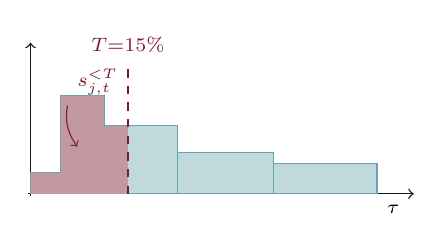
\begin{tikzpicture}[font=\small, xscale=0.55, yscale=0.48]
  \def\pa{0.7}
  \def\pb{1.7}
  \def\pc{3.4}
  \def\pd{5.6}
  \def\pe{8.0}
  \def\Tx{2.25}

  \draw[->, Navy, line width=0.5pt] (-0.05,0) -- (8.85,0);
  \draw[->, Navy, line width=0.5pt] (0,-0.05) -- (0,4.0);
  \node[font=\scriptsize, anchor=north east] at (8.75,-0.03) {$\tau$};

  \fill[Teal!30, draw=Teal!70, line width=0.4pt] (0,0) rectangle (\pa, 0.55);
  \fill[Teal!30, draw=Teal!70, line width=0.4pt] (\pa,0) rectangle (\pb, 2.6);
  \fill[Teal!30, draw=Teal!70, line width=0.4pt] (\pb,0) rectangle (\pc, 1.8);
  \fill[Teal!30, draw=Teal!70, line width=0.4pt] (\pc,0) rectangle (\pd, 1.1);
  \fill[Teal!30, draw=Teal!70, line width=0.4pt] (\pd,0) rectangle (\pe, 0.8);

  % Red overlay for low-taxed
  \fill[Bordeaux!45] (0,0) rectangle (\pa, 0.55);
  \fill[Bordeaux!45] (\pa,0) rectangle (\pb, 2.6);
  \fill[Bordeaux!45] (\pb,0) rectangle (\Tx, 1.8);

  \draw[Bordeaux, dashed, line width=0.8pt] (\Tx,0) -- (\Tx,3.45);
  \node[font=\scriptsize, Bordeaux, anchor=south] at (\Tx,3.48) {$T{=}15\%$};

  \node[font=\scriptsize, Bordeaux, align=left] (slowtax) at (1.55,2.95) {$s_{j,t}^{<T}$};
  \draw[->, Bordeaux, line width=0.4pt] (slowtax.south west) to[bend right=20] (1.08, 1.25);
\end{tikzpicture}
\end{column}
\end{columns}
\end{frame}

\note{
Stage 1 in more detail. The jurisdiction-average approach treats a country as either entirely above or below 15 percent. The distributional approach fits a piecewise-uniform density from the five CbCR percentiles and integrates below the threshold. The red area in the graph is the low-taxed share. Switching from average to distributional roughly doubles the measured GMT base. This is the single biggest modelling choice, and it is Factor 1 in my design.
}


\begin{frame}{Stage 2: the SBIE erodes the effective floor}
\begin{center}
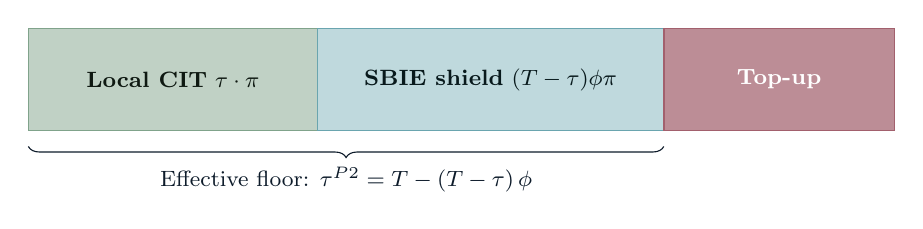
\begin{tikzpicture}[font=\small]
  \def\W{11}
  \def\H{1.3}
  \def\xa{3.67}
  \def\xb{8.07}

  \fill[ForestGreen!35, draw=ForestGreen!70, line width=0.5pt] (0,0) rectangle (\xa, \H);
  \node[font=\footnotesize, ForestGreen!20!black] at (\xa/2, \H/2) {\textbf{Local CIT} $\tau \cdot \pi$};

  \fill[Teal!30, draw=Teal!70, line width=0.5pt] (\xa,0) rectangle (\xb, \H);
  \node[font=\footnotesize, Teal!20!black] at ({(\xa+\xb)/2}, \H/2) {\textbf{SBIE shield} $(T-\tau)\phi\pi$};

  \fill[Bordeaux!50, draw=Bordeaux!70, line width=0.5pt] (\xb,0) rectangle (\W, \H);
  \node[font=\footnotesize, white] at ({(\xb+\W)/2}, \H/2) {\textbf{Top-up}};

  \draw[decorate, decoration={brace, mirror, amplitude=4pt}, Navy]
    (0,-0.2) -- node[below=4pt, font=\footnotesize]
    {Effective floor: $\tau^{P2} = T - (T - \tau)\,\phi$} (\xb,-0.2);
\end{tikzpicture}
\end{center}

\vspace{0.5em}
\begin{columns}[T]
\begin{column}{0.48\textwidth}
  \textbf{Devereux (2023):}\\[3pt]
  Average $\phi = 57\%$ at initial rates\\
  $\to$ effective floor is \emphbx{6.45\%}, not 15\%\\[6pt]
  At long-run rates: $\phi = 41\%$\\
  $\to$ effective floor rises to 8.85\%
\end{column}
\begin{column}{0.48\textwidth}
  \textbf{Schjelderup (2024):}\\[3pt]
  The SBIE acts as a \emph{de facto} production subsidy\\[6pt]
  Capital-intensive sectors benefit most\\[6pt]
  $\to$ heterogeneous impact across EU sectors
\end{column}
\end{columns}
\end{frame}

\note{
Stage 2. The SBIE shields profit backed by payroll and tangible assets. Devereux finds an average SBIE-to-profit ratio of 57 percent, so the effective minimum tax is only 6.45 percent in year one, not 15 percent. Schjelderup shows it acts as a production subsidy favouring capital-intensive sectors. This is why the sectoral decomposition with FATS matters: the aggregate SBIE conceals dramatic variation across sectors.
}


\begin{frame}{Stage 3: panel estimation of the semi-elasticity}

The Hines--Rice framework adapted to the CbCR panel:

$$\log \pi_{p,j,t}^{*} = \beta_0 + \beta_1 \log A + \beta_2 \log \hat{W} + f(\tau) + \boldsymbol{\beta}_x \mathbf{X} + \alpha_{pj} + \gamma_t + \varepsilon$$

\vspace{0.3em}
Three functional forms for $f(\tau)$:

\vspace{0.3em}
\begin{center}
\small
\begin{tabular}{@{}lll@{}}
  \toprule
  \textbf{Form} & $f(\tau)$ & \textbf{Semi-elasticity} $\varepsilon(\tau)$ \\
  \midrule
  Linear & $\beta_3 \tau$ & $\beta_3$ \quad (constant) \\[4pt]
  Quadratic & $\beta_3 \tau + \beta_4 \tau^2$ & $\beta_3 + 2\beta_4 \tau$ \quad (bounded) \\[4pt]
  Logarithmic & $\beta_3 \tau + \beta_4 \log(t_0 + \tau)$ & $\beta_3 + \beta_4/(t_0 + \tau)$ \quad (\emphbx{unbounded}) \\
  \bottomrule
\end{tabular}
\end{center}

\vspace{0.5em}
\highlight{Key:} $\alpha_{pj}$ absorbs all time-invariant bilateral confounders. Identification from \emph{within-pair} ETR variation over 2016--2022.
\end{frame}

\note{
Stage 3. I use the Hines-Rice framework with the CbCR panel. Log corrected profit on the left, real-activity controls and a tax function on the right. The pair fixed effect alpha-pj absorbs all time-invariant bilateral confounders: treaty networks, group structure, everything. Identification comes from within-pair ETR variation over seven years. Three functional forms: linear gives a constant semi-elasticity, quadratic is bounded at zero, logarithmic rises without bound. Only the logarithmic captures the extreme nonlinearity at low rates. I compare them on BIC and rank. The instrument for the ETR is the lagged statutory rate, to handle division bias.
}


%% ═══════════════════════════════════════════════
\section{Expected Findings \& Hypotheses}
%% ═══════════════════════════════════════════════

\begin{frame}{Five hypotheses}
\begin{enumerate}
  \item[\textbf{H1}] The logarithmic specification dominates; $\hat{\varepsilon}(0.05)$ exceeds 0.8 by at least a factor of three.

  \item[\textbf{H2}] ETR measurement (Factor 1) accounts for the \highlight{largest share} of variance in the ANOVA.

  \item[\textbf{H3}] Factor interactions $\geq$ 10\% of total variance. One-at-a-time sensitivity \emphbx{understates} the true range.

  \item[\textbf{H4}] The SbS Safe Harbour reduces EU IIR/UTPR revenue; turns it \emphbx{negative} for countries without QDMTT.

  \item[\textbf{H5}] The SBTI Safe Harbour reduces the effective floor heterogeneously; largest in \highlight{capital-intensive} sectors.
\end{enumerate}
\end{frame}

\note{
Five testable hypotheses. H1: the logarithmic form wins on BIC and the semi-elasticity at 5 percent is at least 2.4, three times the consensus. H2: ETR measurement is the single biggest factor. H3: interactions are at least 10 percent of variance, which means you cannot do one-at-a-time sensitivity. H4: SbS cuts IIR and UTPR revenue, possibly turning it negative for countries without a QDMTT. H5: the SBTI Safe Harbour benefits capital-intensive sectors disproportionately. Each hypothesis maps to a subquestion and has a clear rejection criterion.
}


%% ═══════════════════════════════════════════════
\section{Timeline}
%% ═══════════════════════════════════════════════

\begin{frame}{Period 4 timeline: April--June 2026}
\begin{center}
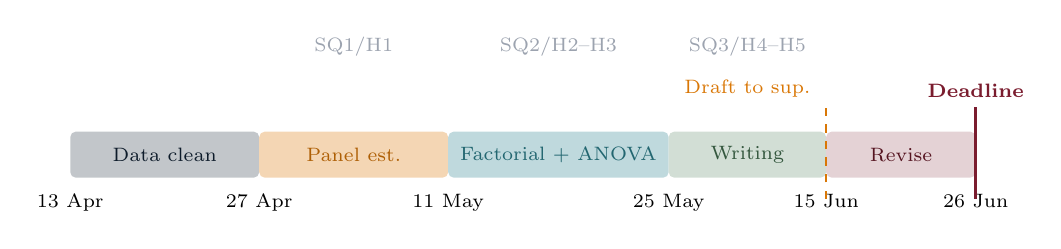
\begin{tikzpicture}[font=\small, xscale=1.0, yscale=0.9]
  \def\ybase{0}
  \def\bh{0.65}

  % Phase bars
  \fill[Navy!25, rounded corners=2pt] (0,\ybase) rectangle (2.4, \ybase+\bh);
  \fill[DkOrange!30, rounded corners=2pt] (2.4,\ybase) rectangle (4.8, \ybase+\bh);
  \fill[Teal!30, rounded corners=2pt] (4.8,\ybase) rectangle (7.6, \ybase+\bh);
  \fill[ForestGreen!25, rounded corners=2pt] (7.6,\ybase) rectangle (9.6, \ybase+\bh);
  \fill[Bordeaux!20, rounded corners=2pt] (9.6,\ybase) rectangle (11.5, \ybase+\bh);

  % Labels inside bars
  \node[font=\scriptsize, Navy] at (1.2, \ybase+\bh/2) {Data clean};
  \node[font=\scriptsize, DkOrange!80!black] at (3.6, \ybase+\bh/2) {Panel est.};
  \node[font=\scriptsize, Teal!80!black] at (6.2, \ybase+\bh/2) {Factorial + ANOVA};
  \node[font=\scriptsize, ForestGreen!70!black] at (8.6, \ybase+\bh/2) {Writing};
  \node[font=\scriptsize, Bordeaux!70!black] at (10.55, \ybase+\bh/2) {Revise};

  % Date labels below
  \node[below, font=\scriptsize] at (0, \ybase-0.1) {13 Apr};
  \node[below, font=\scriptsize] at (2.4, \ybase-0.1) {27 Apr};
  \node[below, font=\scriptsize] at (4.8, \ybase-0.1) {11 May};
  \node[below, font=\scriptsize] at (7.6, \ybase-0.1) {25 May};
  \node[below, font=\scriptsize] at (9.6, \ybase-0.1) {15 Jun};
  \node[below, font=\scriptsize] at (11.5, \ybase-0.1) {26 Jun};

  % SQ mapping (top row, well above bars)
  \node[font=\scriptsize, MidGrey] at (3.6, \ybase+\bh+1.2) {SQ1/H1};
  \node[font=\scriptsize, MidGrey] at (6.2, \ybase+\bh+1.2) {SQ2/H2--H3};
  \node[font=\scriptsize, MidGrey] at (8.6, \ybase+\bh+1.2) {SQ3/H4--H5};

  % Milestone markers (below SQ labels)
  \draw[DkOrange, line width=0.8pt, dashed] (9.6, \ybase-0.3) -- (9.6, \ybase+\bh+0.35);
  \node[above, font=\scriptsize, DkOrange] at (8.6, \ybase+\bh+0.35) {Draft to sup.};

  \draw[Bordeaux, line width=1.2pt] (11.5, \ybase-0.3) -- (11.5, \ybase+\bh+0.35);
  \node[above, font=\scriptsize\bfseries, Bordeaux] at (11.5, \ybase+\bh+0.35) {Deadline};
\end{tikzpicture}
\end{center}

\vspace{0.8em}
\begin{itemize}
  \item All raw data already downloaded and analysed at first-stage level
  \item Methodology worked out in detail (extensive working document)
  \item One-week buffer before final deadline
\end{itemize}
\end{frame}

\note{
The timeline. First two weeks: finalise data cleaning. Then two weeks panel estimation. Then two weeks factorial design and ANOVA. Then writing and the SbS analysis. Draft to supervisor around 15 June, final deadline 26 June. All raw data are already downloaded and the methodology is worked out in a much longer working document. I have a one-week buffer at the end.
}


%% ═══════════════════════════════════════════════
%%  CLOSING SLIDE
%% ═══════════════════════════════════════════════
{
\setbeamercolor{background canvas}{bg=Navy}
\begin{frame}[plain]
  \vspace{2.5em}
  \begin{center}
    {\color{Ivory}\Large\bfseries Thank you}\\[1.2em]
    {\color{DkOrange}\rule{4cm}{2pt}}\\[1.2em]
    {\color{WarmGrey}\normalsize Questions?}\\[2.0em]
    {\color{MidGrey}\small Maurits de Haan $\cdot$ m.c.p.dehaan@students.uu.nl}
  \end{center}
\end{frame}
}


%% ═══════════════════════════════════════════════
%%  BACKUP SLIDES
%% ═══════════════════════════════════════════════
\appendix

{
\setbeamercolor{background canvas}{bg=MidNavy}
\begin{frame}[plain]
  \vfill
  \centering
  {\color{Ivory}\LARGE\bfseries Backup Slides}\\[0.6em]
  {\color{DkOrange}\rule{4cm}{2pt}}
  \vfill
\end{frame}
}


\begin{frame}{Backup: the SBIE formula and effective floor}
The SBIE for each bilateral pair:
$$\text{SBIE}_{p,j,t} = \sigma_W(t) \cdot \hat{W}_{p,j,t} + \sigma_A(t) \cdot A_{p,j,t}$$

Carve-out rates decline over the transition:

\vspace{0.3em}
\begin{center}
\small
\begin{tabular}{@{}lcc@{}}
  \toprule
  & \textbf{Payroll} $\sigma_W$ & \textbf{Assets} $\sigma_A$ \\
  \midrule
  Year 1 (2024) & 10\% & 8\% \\
  Year 10 (2033) & 5\% & 5\% \\
  \bottomrule
\end{tabular}
\end{center}

\vspace{0.4em}
Effective floor: $\tau^{P2} = T - (T - \tau)\,\phi$, where $\phi = \text{SBIE}/\pi$\\[6pt]
Devereux: average $\phi = 0.57$ $\to$ effective floor = 6.45\%\\
At long-run rates: $\phi = 0.41$ $\to$ effective floor = 8.85\%
\end{frame}


\begin{frame}{Backup: the counterfactual profit under the GMT}
For the logarithmic specification, counterfactual profit:
$$\hat{\pi}_{p,j,t}^{\text{GMT}} = \pi_{p,j,t}^{*} \cdot \exp\!\left[\hat{\beta}_3 (T - \tau) + \hat{\beta}_4 \bigl(\log(t_0 + T) - \log(t_0 + \tau)\bigr)\right]$$

The behavioural filter:
$$\beta_{j,t} = 1 - \frac{\hat{\pi}_{j,t}^{\text{GMT}}}{\pi_{j,t}^{*}}$$

\vspace{0.5em}
\textbf{Identification concern:} division bias ($\tau = \theta/\pi$, shock to $\pi$ mechanically lowers $\tau$).\\[4pt]
\textbf{Solution:} instrument with lagged statutory CIT rate. Policy-driven, not mechanically affected by same-year MNE shifting.
\end{frame}


\begin{frame}{Backup: profit-base correction for double counting}
CbCR profits are overstated by 47--72\% due to intra-group dividends (Blouin 2023; Garcia-Bernardo 2022).\\[8pt]

Correction strategy:
$$\gamma_j = \alpha + \beta \cdot \frac{\text{ACT\_HOLDING}_j}{\text{ENTITIES\_COUNT}_j} + \varepsilon_j$$

\begin{itemize}
  \item Use \texttt{PROFIT\_ADJ} where available (2021--2022)
  \item Predict correction ratio for 2016--2020 using holding-company intensity
  \item Hypothesis: $\beta < 0$ (more holdings $\to$ more double counting)
\end{itemize}
\end{frame}


\begin{frame}{Backup: the Side-by-Side Safe Harbour}
January 2026 OECD Administrative Guidance:
\begin{itemize}
  \item \textbf{SbS:} US-parented MNE groups exempted from IIR and UTPR collection
  \item Only the QDMTT channel remains for those groups
  \item EU countries \emphbx{without a QDMTT} lose all collection on US-parented groups
\end{itemize}

\vspace{0.5em}
\textbf{SBTI Safe Harbour:}
\begin{itemize}
  \item Qualifying tax incentives can be added to covered taxes
  \item Bounded by a Substance Cap tied to payroll and assets
  \item $\to$ capital-intensive sectors benefit most (Schjelderup 2024)
\end{itemize}

\vspace{0.5em}
\textbf{The Dutch case:} SbS reduced projected revenue by around \EUR120m/year.
\end{frame}


\begin{frame}{Backup: CbCR Table structure overview}
\begin{center}
\footnotesize
\begin{tabular}{@{}lL{2.5cm}L{2.5cm}L{2.5cm}L{3cm}@{}}
  \toprule
  & \textbf{Table I} & \textbf{Table II} & \textbf{Table III} & \textbf{Table IV} \\
  \midrule
  Content & Agg.\ totals + percentiles & Interquartile means & ETR brackets (MNE) & ETR brackets (subsidiary) \\
  Rows & 1.12m & 437k & 699k & 101k \\
  Parents & 58 & 46 & 46 & 49 \\
  Affiliates & 240 & 238 & 238 & 154 \\
  Key use & Distributional fit & Robustness check & Activity composition & Direct GMT base \\
  \bottomrule
\end{tabular}
\end{center}

\vspace{0.4em}
{\footnotesize Tables V and VI: size distribution and 2022 size-class disaggregation (supporting roles).}
\end{frame}


\begin{frame}{Backup: cross-validation of distributional fit}
Three tests on the Table I $\cap$ Table IV overlap sample:

\vspace{0.4em}
\begin{enumerate}
  \item \textbf{Low-taxed share:} $s^{<T,\text{I}}$ vs.\ $s^{<T,\text{IV}}$ \\
    Wilcoxon signed-rank test for systematic bias

  \item \textbf{Bracket fit:} total variation distance
    $$\text{TV}_{j,t} = \tfrac{1}{2}\sum_{b} \left|\hat{\omega}^{\text{I}}_{j,t,b} - \omega^{\text{IV}}_{j,t,b}\right|$$

  \item \textbf{Revenue impact:} regress percentage revenue difference on ETR IQR
    $$\frac{R^{\text{I}} - R^{\text{IV}}}{R^{\text{IV}}} = \alpha + \delta \cdot \text{IQR}^{\text{ETR}} + \gamma_t + \varepsilon$$
    If $\hat{\delta} \approx 0$: distributional approach is approximately unbiased.
\end{enumerate}
\end{frame}


\begin{frame}{Backup: two types of uncertainty}
The thesis separates:

\vspace{0.5em}
\begin{columns}[T]
\begin{column}{0.47\textwidth}
\begin{block}{Scenario spread}
  Range across 32 configurations (holding semi-elasticity at point estimate).\\[4pt]
  Driven by \emph{assumptions} --- more data cannot resolve it.
\end{block}
\end{column}
\begin{column}{0.47\textwidth}
\begin{block}{Estimation uncertainty}
  Bootstrapped 90\% CI within a single scenario.\\[4pt]
  Driven by \emph{statistical precision} --- shrinks with more data.
\end{block}
\end{column}
\end{columns}

\vspace{0.8em}
Their ratio:
$$\Lambda_{j,t} = \frac{\max_{\mathbf{x}} R(\mathbf{x}) - \min_{\mathbf{x}} R(\mathbf{x})}{q_{0.95}(R^*) - q_{0.05}(R^*)}$$

$\Lambda > 1$: assumptions matter more than data.\\
$\Lambda < 1$: collect more data, it will help.
\end{frame}


\begin{frame}{Backup: Johannesen welfare thresholds}
Johannesen (2022): GMT is welfare-improving only when the semi-elasticity is sufficiently high.

\vspace{0.5em}
\begin{center}
\small
\begin{tabular}{@{}lc@{}}
  \toprule
  \textbf{Scenario} & \textbf{Required $\varepsilon$} \\
  \midrule
  Low marginal social value of public funds & $\sim$1.8 \\
  High marginal social value & $\sim$4.2 \\
  Consensus (Heckemeyer \& Overesch) & 0.8 \\
  Dowd quadratic at 5\% & 4.7 \\
  \bottomrule
\end{tabular}
\end{center}

\vspace{0.5em}
The consensus of 0.8 falls below \emph{all} thresholds.\\
The nonlinear estimates at low rates exceed them.\\[4pt]
$\to$ \highlight{Which semi-elasticity you use determines whether the GMT passes the welfare test.}
\end{frame}


\begin{frame}{Backup: Swiss anomaly in Table IV}
Switzerland data in Table IV is anomalous in 2017, 2020, 2022:
\begin{itemize}
  \item Reported profit approximately 8,600$\times$ Table I levels
  \item Likely a reporting or classification error
  \item CHE excluded from those vintage-years in the estimation
\end{itemize}

\vspace{0.5em}
Robustness check: include CHE with winsorisation. Results should be insensitive if the exclusion is justified.
\end{frame}


\begin{frame}{Backup: collection channels --- QDMTT, IIR, UTPR}
\begin{center}
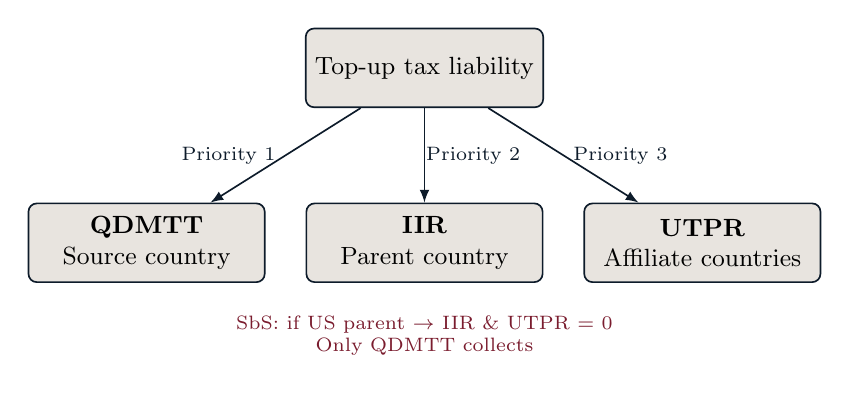
\begin{tikzpicture}[font=\small, node distance=0.7cm]
  \tikzset{
    ch/.style={draw=Navy, rounded corners=3pt, fill=WarmGrey, minimum width=3cm,
               minimum height=1.0cm, align=center, line width=0.6pt},
    arr/.style={-latex, Navy, line width=0.6pt}
  }

  \node[ch] (topup) {Top-up tax liability};
  \node[ch, below left=1.2cm and 0.5cm of topup] (qdmtt) {\textbf{QDMTT}\\Source country};
  \node[ch, below=1.2cm of topup] (iir) {\textbf{IIR}\\Parent country};
  \node[ch, below right=1.2cm and 0.5cm of topup] (utpr) {\textbf{UTPR}\\Affiliate countries};

  \draw[arr] (topup) -- (qdmtt) node[midway, left, font=\scriptsize] {Priority 1};
  \draw[arr] (topup) -- (iir) node[midway, right, font=\scriptsize, xshift=-3pt] {Priority 2};
  \draw[arr] (topup) -- (utpr) node[midway, right, font=\scriptsize] {Priority 3};

  \node[font=\scriptsize, Bordeaux, below=0.3cm of iir, align=center]
    {SbS: if US parent $\to$ IIR \& UTPR = 0\\Only QDMTT collects};
\end{tikzpicture}
\end{center}
\end{frame}




\end{document}
